\documentclass[./Research.tex]{subfiles}

\begin{document}

Possibly the simplest two computations to combine into a single network are addition and subtraction. This can be accomplished using a syntax tree-style structure where an eval function is given an operator and two inputs. For example, the eval function would evaluate "+ 5 4" to 9, or "- 5 4" to 1.

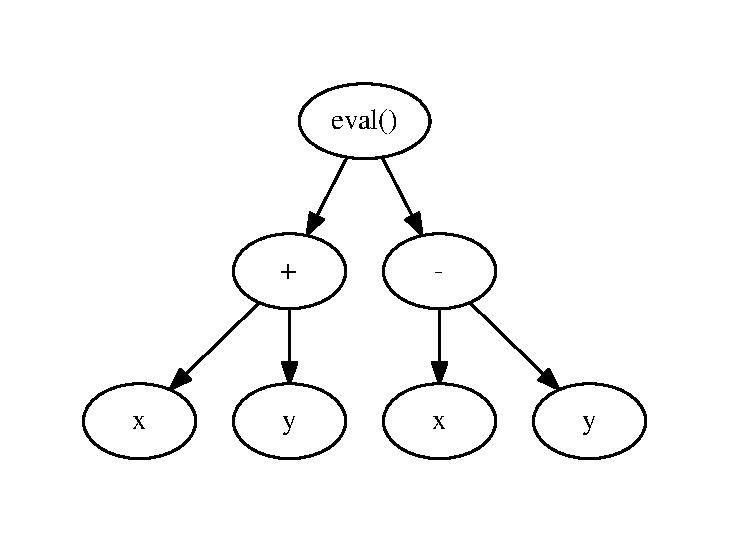
\includegraphics{Visuals/NeuralNetwork_1_SyntaxTree.pdf}

This structure is very similar to how compilers/interpreters view and evaluate code in a program.

\end{document}
